\section{Entorno de desarrollo}\label{sec:entorno}

\todo{explicación general sobre VSCode y plugin de lean}

\subsection*{Símbolos matemáticos}

Como se ha mencionado anteriormente en este documento, en \textit{Lean} se
pueden utilizar símbolos unicode para expresar tipos útiles en la formalización
de matemáticas y obtener así un código más cercano a las notaciones lógicas a
las que estamos acostumbrados a usar en matemáticas.

La inclusión de estos caracteres está facilitada en el entorno de
desarrollo, escribiendo comandos que empiecen por \texttt{\textbackslash} estos
se reemplazarán por el caracter correspondiente. Por ejemplo al escribir
\texttt{\textbackslash to} este comando se reemplazará automáticamente por el
caracter \lstinline{→}, \texttt{\textbackslash lambda} por \lstinline{λ} y
\texttt{\textbackslash N} por \lstinline{ℕ}.

\subsection*{Panel de estado táctico}

\todo{redactar}

\begin{figure}[htbp]
	\centerline{\frame{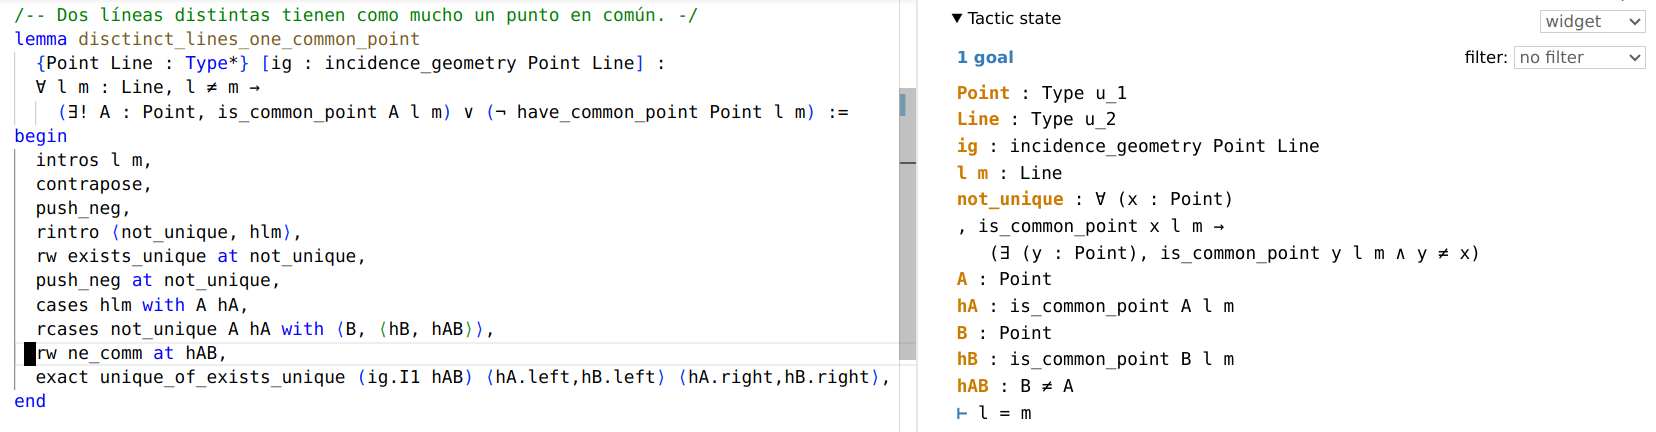
\includegraphics[width=17cm]{./imgs/captura.png}}}
	\caption*{Captura de pantalla del entorno de dearrollo en el editor \textit{Visual Studio Code}.}
	\label{figure:entorno}
\end{figure}



